
\begin{figure}
\figurefontsize
\centering
%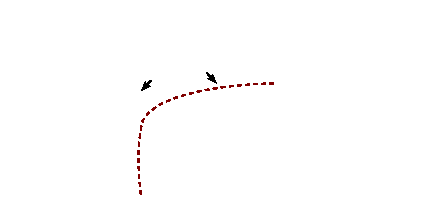
\includegraphics[width=3.00in,height=1.50in]{Fig/valveSharing.eps}
\input{Fig/valveSharing.pdf_tex}
\caption{Valve sharing and its interfering with test and application execution.}
\label{fig:valveSharing}
\end{figure}

\section{Valve Sharing in Test and Application
Execution}\label{sec:valve_sharing}

In implementing single-source single-meter test for a multi-port
biochip, new DFT channels and valves are added into the chip architecture. The
newly added DFT valves also require control signals that switch them open or
closed to regulate the fluid transportation. These control signals are also
air pressure conducted to valves through control channels. If the newly added
DFT valves are controlled independently, both control channels and 
external air pumps should be added, leading to an increase of the cost for manufacturing
and running the chip.  In this section, we propose a valve-sharing technique
which eliminates the control overhead by sharing the control signals of
DFT valves with those for original valves, while maintaining the performance
of the chip.

\subsection{Valve Sharing and its Validation}\label{sec:validation}

Figure~\ref{fig:valveSharing} demonstrates how valves share controlling
channels in a DFT architecture, where each new valve is connected to the
control channel that is already existing to control another valve in the
original chip.  In this example, the DFT valve $v_0$ shares its control
channel with $v_3$ and the DFT valve $v_2$ shares its control channel with
$v_1$.  Consequently, $v_0$ and $v_3$ always open and close simultaneously,
and so do $v_2$ and $v_1$. This sharing scheme, however, interferes with the
test procedure as well as the execution of the application.  Therefore, we
need to develop methods to validate a valve sharing scheme before exploring the
design space of valve sharing.

%\subsubsection{Validation of valve sharing for testing}

Assume that $v_1$ and $v_3$ are kept closed during test to form a cut to
separate the pressure source and the pressure meter.  If $v_3$ cannot be
closed properly due to defects, it is supposed that the pressure 
meter should be able to measure
the leaked air pressure. However, with valve sharing shown in
\figname~\ref{fig:valveSharing}, $v_0$ is also closed, masking the error
supposed to be detected by this cut.

To validate whether a given valve sharing scheme is valid for the test
procedure, each test vector, either a test path or a test cut, is applied
and the output at the pressure meter is verified. For example, in the
case in \figname~\ref{fig:valveSharing}, the validation can be performed
by checking whether there is still a path from the pressure source to the
meter after the test cut is activated and a valve, e.g., $v_3$, cannot be
closed properly. 

Similarly, valve sharing may also affect the execution of an application.
Assume a transportation of fluid is performed from device $d_0$ to device
$d_1$ through the upper path, so that $v_0$ must be opened. However, 
$v_3$ is also opened due to valve sharing, leading to a fluid leakage at $d_1$.

The validation of a valve sharing scheme during application execution is similar
to the case for test. In a given schedule of an application, 
%the device and channel occupation at every moment is known.  
the occupation of all devices and channels at every moment are known. 
These snapshots of
chip occupation are examined together with the given valve sharing scheme
to check whether all the operations can be performed correctly.

\subsection{DFT with Valve Sharing using Particle Swarm Optimization (PSO)}

As discussed above, DFT augmentation brings new channels and valves into
the chip. Not only the locations of added channels and valves but also the
control sharing scheme affect the test procedure and the execution of the
application. In the proposed method, we deploy the Particle Swarm Optimization
(PSO) algorithm to find valid DFT architectures that still maintain the
efficiency of application execution.

Particle swarm optimization (PSO) is a stochastic population-based
optimization algorithm \cite{pso95}. Members of the population (swarm) are
called particles.  At the beginning of the algorithm, particles are randomly
scattered into the whole search space. A particle $p_i$ possesses a position
$x_i$. A random velocity $v_i$ is assigned to particle $p_i$ and a cost
function is applied for each particle to assess the quality of its current
location.  For each particle $p_i$, a local best position $p_{best,i}$ in its
search history is tracked. For the whole swarm, a global best position
$g_{best}$ with the best assessment of all particles is also recorded.  In
each iteration, the new velocity and position of a particle $p_i$ are updated
as follows
\begin{align}\label{eq:pso_update}
v_i = \omega * v_i + c_1*rand_1*(x_i - p_{best,i})+c_2*rand_2*(x_i-g_{best}) \\
x_i = x_i + v_i 
\end{align}
where $\omega$, $c_1$ and $c_2$ are constants to control the search speed.
$rand_1$ and $rand_2$ are two random numbers to incorporate
stochasticity into the search iterations.
%P is the set of all particles. 
After each iteration, the performance at the new position of each particle
and the global assessment are updated.

%PSO makes each particle moves around in the search space, taking advantage of
%the particle’s own experience and the experience of the particle’s neighbours
%or of the whole swarm to guide the search.

%PSO needs a swarm of particles and their initial positions.  
In the proposed method, the
%initial 
position of a particle consists of two parts of information: 1) how to add new channels
to meet the single-source single-meter requirements; 2)
how new valves share control channels with original valves. 
Therefore, we use two multidimensional vectors to denote these positions.
%two parts of information.

In Section~\ref{sec:dft_arch}, the optimization problem
(\ref{eq:DFT_opt_1})--(\ref{eq:DFT_opt_2}) may produce  many viable solutions
to meet the constraints and the objective.
%specially the the minimization objective is  Therefore, we can use different
%edges combination to construct additional channels to meet DFT requirements. 
A vector $\vec{X}^{a}= [x_0,x_1,...,x_n]$ is thus used to denote which edges
in the connection grid are used to construct new channels.  The definition of
$x_i$ is as follows.
\begin{equation}
  x_i =
  \begin{cases}
    1 & \text{if $e_i$ in the connection grid 
      is used for DFT;}\\
    0 & \text{otherwise}
  \end{cases}
\end{equation}
where $e_i$ represents an edge in the connection grid in \figname~\ref{fig:fitintogrid}.
%where $n$ is the number of possible edges to construct a DFT architecture in a connection grid.

%Knowing the locations of new edges added for DFT, we can also deduce the
%locations of valves at the crossing points of channels. 
For valve sharing, assume that the number
of valves for DFT is $n_d$ and the number of valves in the original chip is
$n_v$.  A vector
$\vec{X}^{s}$
is used to denote how DFT valves share control channels with original valves,
defined as
\begin{align}\label{eq:valves_include}
  \vec{X}^{s} =\{x_{i,j}\}, \qquad 0\le i\le n_d, \quad  0\le j\le n_v\\
  x_{i,j}=
  \begin{cases}
    1 & \text{if valve $v_i$ shares control channel with valve $v_j$}; \\
    0 & \text{otherwise.}
  \end{cases}
\end{align}

A PSO particle position is defined as the combination of the two vectors
$\vec{X} = [\vec{X}^{a}, \vec{X}^{s}]$. The quality of a position is evaluated by
two criteria. First, if the locations of DFT channels and valves as well as the
corresponding control sharing scheme cannot pass the validation step described
in Section~\ref{sec:validation}, the quality of this position is set to
$\infty$, meaning that the execution time of the application is so large that
this position is invalid. If this position can pass the validation, its
quality is set to the corresponding execution time of the application at this
position.

In executing the PSO algorithm, valve sharing information can only be obtained
after DFT channels and valves are created. Moreover, the validation of test
and application execution can be performed after the valve sharing scheme is
determined. Only after these steps, the execution time of the application can
be evaluated.  Consequently, multiple phases are required in each PSO
iteration to generate new particle positions and to assess their quality.

In each PSO iteration, for a particle $p_i$ with its position $\vec{X}_i =
[\vec{X}^{a}_i, \vec{X}^{s}_i]$, the operations are as follows. 

\begin{enumerate} 

    %\newlength{\mylength} 
    \setlength\mylength{\parskip}
    \setlength\parskip{-3.5mm}
    %\setlength\itemsep{0.01em}
  \item 

  $\vec{X}^{a}_i$ is updated according to the PSO search strategy, producing a
  new DFT configuration by solving (\ref{eq:DFT_opt_1})--(\ref{eq:DFT_opt_2}).
  \setlength\parskip{\mylength}

  \item 
 % Finding the best share plan in the given $\vec{X^{add}_i}$. In this phase, 
  A sub-PSO algorithm is applied to find the best valve sharing scheme. 
  First, randomized sub-particles with respect to different valve sharing schemes
  are generated. Their positions are set to $\vec{X}^{s}$. 
  Since for each sub-particle, both new channels and valves as well as their
  sharing information are known, we can then assess the quality of these
  positions by validating them using the technique discussed in 
  Section~\ref{sec:validation}. After the sub-PSO algorithm is finished, 
  a valve sharing with the minimum execution time of the application 
  with respect to this sharing scheme is returned. 
  

  \item 

  By combining $\vec{X}^{a}_i$ and its best valve sharing scheme
  $\vec{X}^{s}_i$, we update the quality of the position 
  $\vec{X}_i = [\vec{X}^{a}_i, \vec{X}^{s}_i]$ for $p_i$ with the returned
  application execution time. 

  \item 
    
  After all particles find their new positions and their qualities are assessed,
  the local best position $p_{best,i}$ for particle $p_i$ and the 
  global best position $g_{best}$ are updated accordingly. The iteration goes
  back to step (1) until the maximum allowed number of iterations is reached.

\end{enumerate}

The PSO algorithm returns a DFT architecture together with its valve sharing
scheme. The test vectors and application schedule considering valve sharing
are also generated. The new architecture does not impose
more control overhead, while facilitating the test process and maintaining 
the performance of application execution.

%!!!psuedo code?????
